\documentclass[11pt]{article}
\usepackage[utf8]{inputenc}
\usepackage[T1]{fontenc}
\usepackage{ctex}
\usepackage{float}
\usepackage{graphicx}
\usepackage{longtable}
\usepackage{wrapfig}
\usepackage{rotating}
\usepackage[normalem]{ulem}
\usepackage{amsmath}
\usepackage{amssymb}
\usepackage[binary-units]{siunitx}
\usepackage{capt-of}
\usepackage{imakeidx}
\usepackage{hyperref}
\hypersetup{
    colorlinks=true,
    citecolor=black,
    linkcolor=blue,
    filecolor=magenta,
    urlcolor=cyan,
    pdftitle={OS Case Study},
    pdfpagemode=FullScreen,
    }
\usepackage{xcolor}
\usepackage{tikz}
\usetikzlibrary{trees}
\usepackage{listings}
\definecolor{codegreen}{rgb}{0,0.6,0}
\definecolor{codegray}{rgb}{0.5,0.5,0.5}
\definecolor{codepurple}{rgb}{0.58,0,0.82}
\definecolor{backcolour}{rgb}{0.95,0.95,0.92}
\lstdefinestyle{mystyle}{
    backgroundcolor=\color{backcolour},
    commentstyle=\color{codegreen},
    keywordstyle=\color{magenta},
    numberstyle=\tiny\color{codegray},
    stringstyle=\color{codepurple},
    basicstyle=\ttfamily\footnotesize,
    breakatwhitespace=false,
    breaklines=true,
    captionpos=b,
    keepspaces=true,
    numbers=left,
    numbersep=5pt,
    showspaces=false,
    showstringspaces=false,
    showtabs=false,
    tabsize=2
}
\lstset{style=mystyle}
\usepackage{footmisc}
\usepackage{biblatex}
\usepackage[most]{tcolorbox}
\newtcolorbox{notebox}[0]{colback=yellow!5!white,
colframe=yellow!75!black,fonttitle=\bfseries,parbox=false,breakable,
title={Note}}
\newtcolorbox[auto counter, number within=section, list inside=question]{qbox}[1]{colback=blue!5!white,
colframe=blue!75!black,fonttitle=\bfseries,parbox=false,breakable,
title={小问题~\thetcbcounter:#1}}
\newtcolorbox[auto counter, number within=section, list inside=src]{readsrcbox}[1]{colback=green!5!white,
colframe=green!75!black,fonttitle=\bfseries,parbox=false,breakable,
title={读源码~\thetcbcounter:#1}}
\usepackage{csquotes}

\newcommand{\onlinesrc}[2]{\href{#1#2}{\lstinline{#2}}}
\newcommand{\linuxsrc}[1]
{\onlinesrc{https://git.kernel.org/pub/scm/linux/kernel/git/torvalds/linux.git/tree/}{#1}}
\newcommand{\archlinuxconf}[2]{\href{https://github.com/archlinux/svntogit-packages/blob/974377e2b1ab9e822c71fbb05a82bfb8dd9a7971/trunk/config\#L#1}{#2}}

\addbibresource{bib.bib}
\date{\today}
\title{操作系统案例分析}
\makeindex[intoc, columnseprule, options= -s style.ist]
\begin{document}
\lstset{
	breaklines=true,
	basicstyle=\ttfamily}
\title{OS Case Study}

\maketitle
\tableofcontents

\newpage

\section{历史}
\subsection{Linux 内核的历史}
Linux内核\index{Linux}最初是1991年,当时的赫尔辛基大学本科生Linus Torvalds出于兴趣为自己的386计算机编写的,开发使用的操作系统是教学用的Minix、编译器为GNU的GCC.
当时的背景是这样的:自由软件运动的GNU项目运转了近十年,且取得了很大的进展,GCC作为自由的编译器已经相当成功,其他用户态的工具都比较完善,但是内核项目仍处于早期阶段.
在此之前,Unix于1970年发布,它的成功使得学界和商业界都乐于借鉴其模式和思想.
因此作为一本操作系统教材的配套实现,Minix部分使用了Unix的理念,而GNU也把开发出与Unix兼容的自由操作系统为目标.
Linux 0.1版本发布后,世界上许多开发者对Linus的操作系统很感兴趣,他们加入了Linux的内核的开发,并将一些GNU系统的组件移植到Linux内核,最终使之成为GNU系统事实上的内核.

1992年Linus将Linux 0.99 在GNU General Public License 下发布,Linux正式成为自由软件.

2000年左右,在以著名的论文The Cathedral and the Bazaar为代表的开源运动的影响下,Linux作为开源软件的开发模式开始得到许多公司的重视.
许多硬件和软件公司在这时都开始为Linux提供支持,并加入Linux内核的开发.

如今(2020s)绝大多数互联网服务器运行Linux 发行版\cite{OSUsageT34:online},Linux内核也广泛用于嵌入式设备和智能手机.
作为成熟的可移植的自由类Unix内核,Linux既成为了开源运动的成功范例又为自由软件运动作出了突出的贡献.
\subsection{发行版Arch Linux}
Arch Linux \index{Arch Linux}是程序员兼吉他手Judd Vinet在2002年创建的一个滚动发行的Linux发行版.
其主要特点在于拥有可以自动管理依赖的包管理器pacman和受FreeBSD启发的包构建系统\cite{DistroWa81:online}.
由于Arch Linux上构建和分享软件包非常简单,Arch Linux用户可以使用的软件包非常丰富.
其简易性和以用户为中心\cite{ArchLinux15:online} 的优点使其成为滚动发行模式的代表和最受桌面用户欢迎的Linux发行版之一.

Arch Linux用户可以选择和配置自己的Linux内核,一般使用的是最新的stable分支上的普通的Linux内核.
\begin{notebox}
	由于发行版的内核可以自己配置,发行版的区别对于本案例分析的影响不大,后文的分析将不太涉及发行版之间的区别.
\end{notebox}


\section{Linux内核的架构}
Linux是宏内核,即整个内核是一个共用地址空间的二进制程序.
宏内核架构是相对于微内核而言的.
微内核架构基于消息传递,作为内核的二进制程序只有最基本的功能,其他的不同组件处于不同的地址空间,它们之间通过消息传递的方式来进行交互.
Linux内核采用宏内核的架构主要是出于性能方面的考虑.\cite{silberschatz2021operating}
同一地址空间的各个部分可以直接相互调用,没有消息传递的开销.

宏内核的架构不代表Linux内核不能采用模块化的设计,这得益于动态链接技术.
Linux内核由常驻内存的内核镜像\lstinline{vmlinux}和动态加载的各种模块构成.
使用运行时加载的模块的好处有很多.
首先,这些模块在加载后就处于核心态,可以调用内核中的任何代码,访问硬件也没有限制,这可以使内核的设计者适度地划分各个功能之间的界限——避免功能之间耦合度过高的同时也不必在不同部分之间使用复杂的交互方法.
其次,动态加载模块可以在操作系统运行时更改内核,这对内核的开发有好处,因为不用编译整个内核并重启系统.
这也对节约资源有好处,因为可以只按需要加载内核模块,减少内存占用.

\begin{qbox}{为什么叫“镜像”?}
	\lstinline{vmlinux} 被称为内核“镜像”(kernel image),是因为这个文件在加载操作系统时被用来在内存中创建内核的副本.
	详见Image一词的含义\cite{imageWik70:online}.
\end{qbox}

要了解Linux如何实现模块化的宏内核架构,我们在案例分析中重点介绍两方面的内容:内核模块是如何构建的、内核模块是如何加载的.

\subsection{内核构建系统}
\begin{readsrcbox}{Kernel Build System}
	内核的构建系统有关的文档在 \href{https://docs.kernel.org/kbuild/index.html}{\lstinline{Documentation/kbuild}} 目录.

	可以参考顶层目录的\lstinline{Makefile},各个目录下的\lstinline{Makefile}、\lstinline{Kbuild}.
	另外,\lstinline{script}目录下有用来链接 \lstinline{vmlinux}和有关构建模块的脚本.
\end{readsrcbox}
\begin{qbox}{如何找到某个子系统的有关文件和信息?}
	\lstinline{Maintainer} 文件中列出了Linux内核各个子系统的维护者,同时它还包括有关项目的网页和涉及的文件等有用的信息.
\end{qbox}
Linux内核的构建系统是一套基于GNU Make的递归式的构建系统,包括各个目录下的Makefile和为这些Makefile提供基础设施支持的其他文件,通常称为 \lstinline{kbuild}. \cite{LinuxKer71:online}

整个内核构建系统的目标主要就是内核镜像 \lstinline{vmlinux} 和可加载的模块.
各个Kbuild Makefile以向 \lstinline{obj-m} 和 \lstinline{obj-y} 变量增加内容的方式列出本目录应该构建的目标,
其中 \lstinline{obj-m} 变量中定义的目标会被构建成内核模块——后缀名为 \lstinline{.ko} 的一种ELF文件,而 \lstinline{obj-y} 变量中定义的目标会被 \lstinline{$(AR)}\footnote{一般就是GNU Binutils里面的ar,用于把多个 \lstinline{.o} 目标文件归档到一个文件中.} 合并到一个名为 \lstinline{built-in.a} 的库中,最后被链接进 \lstinline{vmlinux}.
顶层目录的Makefile递归地构建子目录.

有趣的是,内核的各个部分通常既可以编译到内核镜像中,也可以编译成可加载的内核模块,这是由目标是加入到 \lstinline{obj-m} 还是 \lstinline{obj-y} 来决定的.
例如Listing \ref{lst:obj-config}所示,当 \lstinline{CONFIG_BTRFS_FS}的值为y(Yes)时,BTRFS文件系统驱动——目标 \lstinline{btrfs.o}将作为内核内置的一部分编译;
而\lstinline{CONFIG_BTRFS_FS}的值为m(Module)时,它将编译成可加载的内核模块.

\begin{lstlisting}[language=make, caption=可配置的编译目标, label=lst:obj-config]
# fs/btrfs/Makefile
obj-$(CONFIG_BTRFS_FS) := btrfs.o
\end{lstlisting}


\section{进程管理}

\lstinline{struct task_struct} 是Linux内核的进程控制块(PCB).
它存储进程的标识符、进程的状态、指向存储进程上下文的数据结构的指针、调度所需的信息以及与进程相关的资源和指向其他 \lstinline{task_struct} 的指针等.
所有与进程有关的操作都会直接或间接地修改进程控制块来达到目的.
下面,我们介绍管理进程所需要的多种信息,并介绍它们是如何在 \lstinline{task_struct} 中表示的.

\begin{readsrcbox}{进程控制块}
	\lstinline{struct task_struct} 是在\lstinline{include/linux/sched.h}中定义的.
\end{readsrcbox}

首先是进程的状态,一个进程可能处于这些状态:
\begin{itemize}
	\item \lstinline{TASK_NEW}.
	      当一个进程刚创建时,它的状态就被设置为\lstinline{TASK_NEW},表示这个进程已经被创建,但是还没有开始运行.
	\item \lstinline{TASK_DEAD}.
	      进程已经结束.
	\item \lstinline{TASK_RUNNING}.
	      进程正在运行,即该进程在正在运行的进程的队列里.
	\item \lstinline{TASK_INTERRUPTIBLE} 或者 \lstinline{TASK_UNINTERRUPTIBLE}.
	      处于这两个状态的进程正在等待,但是只有 \lstinline{TASK_INTERRUPTIBLE} 状态的进程才会被信号唤醒.
	\item \lstinline{TASK_NOLOAD}.
	      类似 \lstinline{TASK_UNINTERUPTIBLE} 但是在统计数据中不被计入负载.
	      \footnote{\url{https://lore.kernel.org/lkml/alpine.LFD.2.11.1505112154420.1749@ja.home.ssi.bg/T/}}
	\item \lstinline{TASK_WAKING}.
	      进程已经被要求唤醒,但是还没有进入正在运行的进程队列.
	      \footnote{\url{https://lore.kernel.org/lkml/tip-e9c8431185d6c406887190519f6dbdd112641686@git.kernel.org/}}
	\item \lstinline{TASK_WAKEKILL}.
	      该进程收到SIGKILL信号时会被唤醒.
	\item \lstinline{TASK_TRACED}.
	      调试器暂停该进程来追踪它的运行状态.
\end{itemize}
这些状态被编码成掩码,读写进程的状态时,
需要用这些掩码操作 \lstinline{task_struct} 的 \lstinline{__state} 域.
比如识别一个进程是否处于某状态,
就要用它的 \lstinline{__state} 和 这个状态的掩码做与操作,
若结果为0则不处于这个状态.
这些状态中有的状态可以组合成新的掩码,方便使用.

进程控制块还需要存储有关进程上下文的信息,例如有关栈和堆的信息和CPU内部寄存器的值.
这一部分信息既和内核的内存管理有关又依赖于具体的硬件架构.
\begin{readsrcbox}{架构相关代码}
	为了提高可移植性,Linux内核的代码区分不依赖于具体硬件架构的代码和针对特定架构的代码.
	架构相关的代码全部在 \lstinline{arch} 目录下.
	例如 x86和x86\_64的代码位于 \lstinline{arch/x86}.

	显然,所有的汇编代码都应该放在该目录.
	内存管理和进程管理所需的某些功能也依赖于CPU的特定功能,
	需要根据硬件功能定义数据结构和执行具体的指令,
	这些定义和实现也位于 \lstinline{arch} 下具体架构的目录下.
	不同的架构的代码尽量暴露出相同的接口,供架构无关代码使用.

	某一架构上的具体实现的文档可以在 \href{https://docs.kernel.org/arch.html}{\lstinline{Document/arch.rst}} 中的列表找到.
	例如\href{https://docs.kernel.org/x86/kernel-stacks.html}{\lstinline{Document/x86/kernel-stacks.rst}}介绍了x86\_64 CPU上内核为每一个进程维护的若干个栈.
\end{readsrcbox}
\lstinline{task_struct}的定义中,状态后面最先出现的是一个 \lstinline{void *stack;} 域.
这不是该进程的用户态的栈的起始地址,
而是该进程的内核栈,每次该进程通过系统调用进入内核态时,
内核中的代码都在这个内核栈上执行.

Scheduling information is also included in the PCB, including priority of the process, schedule entity that represents the process and a pointer to the schedule class that this process is using.


\section{内存管理} \label{memory management}

Linux的内存管理可以分为内存分配和虚拟内存两个部分.\cite{silberschatz2021operating}
因为Linux采用分页的方式管理内存,内存分配部分的主要任务就是分配物理页、释放物理页.
而虚拟内存部分利用分配出来的物理页来提供内存的抽象,
实现缓存、共享和保护等功能.

\subsection{物理页面的管理}

\subsubsection{物理内存模型}
Linux的内存管理是基于分页技术的,因此物理内存均被看作是页面的数组.
但是物理内存的组织形式又是架构相关的,而且一种架构可以有多种组织方式.
Linux针对不同的物理内存形式,用不同的物理内存模型来管理.
大部分连续的内存对应FLATMEM\index{FLATMEM}模型,
更复杂的内存组织形式对应SPARSEMEM模型.\cite{Physical36:online}
x86-64支持这两种形式,但是FLATMEM不支持非统一内存访问架构(NUMA)\index{NUMA}机器.
Arch Linux和绝大多数x86-64发行版都%
\archlinuxconf{994}{配置}的是SPARSEMEM模型.

SPARSEMEM\index{SPARSEMEM}模型下,物理内存的配置可以很灵活.
物理内存被分段表示,每一个段(section)指向连续存放的一系列物理页面.
内核中管理物理页面的程序\archlinuxconf{995}{可以}存储在动态分配的数组中,
因此甚至可以支持运行时添加内存设备.
配置的灵活性却会给物理内存的访问增加复杂性,
在物理内存不连续的条件下,物理页号(PFN)\index{PFN}并不能用于直接访问真正的物理页.
物理页号到物理页的映射方式有两种,
一种方式是把section的信息编码进PFN中,并且在 \lstinline{struct page}
中也记录section的值.
而默认配置下,例如Arch Linux \archlinuxconf{996}{使用}的是VMEMMAP\index{VMEMMAP} 方式.
这是指在虚拟内存中专门分配一个连续的称作virtual memory map的空间来存放页面信息.
Virtual memory map是页面信息
\lstinline{struct page}\index{p@\lstinline{struct page}}
的一维数组,
以PFN为元素下标,所以要想从PFN找到页面信息(包含页面的物理地址),
只需要计算偏移访问数组即可.
逻辑上,这个数组内有所有的页面的信息,而且是连续的,其大小可与整个物理地址空间的大小相比.
但是,正是因为它是虚拟地址空间的连续数组,而虚拟的页面又可以按需分配,
所以它并不会真正占据很多空间.
这种在物理页面管理中也使用虚拟内存的想法非常能体现虚拟内存的灵活性.

\begin{readsrcbox}{\lstinline{struct page},内存模型}
	\lstinline{struct page} 是存储物理页面的信息的结构体.
	其中包括物理页面的地址,分配和回收页面需要的信息等,
	定义在 \linuxsrc{include/linux/mm_types.h}.

	虚拟地址到物理地址的映射需要用PFN来找到物理页面,
	这就需要用PFN算出对应的 \lstinline{struct page},
	完成PFN和 \lstinline{page} 之间的转换的是宏
	\lstinline{pfn_to_page} 和 \lstinline{page_to_pfn},
	不同的物理内存模型的实现不同,内存模型相关定义可见
	\linuxsrc{include/asm-generic/memory_model.h}.
	其中VMEMMAP由于有虚拟地址上连续的\lstinline{vmemmap},
	其转换过程就是涉及数组元素偏移量的简单计算:
	\begin{lstlisting}[language=C]
/* include/asm-generic/memory_model.h */
#define __pfn_to_page(pfn)	(vmemmap + (pfn))
#define __page_to_pfn(page)	(unsigned long)((page) - vmemmap)
\end{lstlisting}

	SPARSEMEM的VMEMMAP模型下,
	\lstinline{struct page *vmemmap} 由架构相关的代码定义.
	x86-64的位于 \linuxsrc{arch/x86/include/asm/pgtable_64.h}.
	架构无关的用于填充 \lstinline{vmemmap} 的代码位于
	\linuxsrc{mm/sparse-vmemmap.c}.
\end{readsrcbox}

分section的SPARSEMEM内存模型解决了物理内存的差异性,
那么分配页面时如何区分具有不同功能的内存呢?
答案是内存的不同区域还有ZONE的区分.
有些设备不能访问整个地址空间,导致只有一部分地址可以用于直接内存访问DMA\index{DMA}.
这一部分内存被设置为 \lstinline{ZONE_DMA} 或 \lstinline{ZONE_DMA32}.
另外,一些物理地址只是用于访问设备,而不是真正的内存地址,
这些空间被设置为 \lstinline{ZONE_DEVICE},其中的页面永远不会成为空闲页面.
其他的页面都可以用来当作普通的内存来分配,称为 \lstinline{ZONE_NORMAL}.
Linux内核中的物理页面分配代码被称作zoned page allocator,\index{zoned allocator}
是因为每一个zone是被单独管理的,各个zone之间的分配互不干扰.

\subsubsection{页面分配器}

在每一个zone内部,分配器主要实现两个功能:分配页面和释放页面,
即根据调用者的需要找到一定数量的空闲的页面,向调用者返回分配的页面的地址,并把这些页面记录为正在使用,
在调用者使用完这些页面后,再向分配器归还这些页面,使他们重新变为可以分配的空闲页面.

在分配问题\cite{silberschatz2021operating}\index{allocation problem}中,
要避免的是碎片化问题\index{fragmentation}.
页面分配器只关心外碎片化问题\index{external fragmentation},
因为其并不管理页面内部的内存组织方式.
外碎片化问题——无法找到需要的大小的空间即使总的空闲空间能够满足要求\cite{silberschatz2021operating}
——出现的原因是较小的已分配区域散落在不连续的区域中,导致没有大块的空间来满足分配要求.
既然问题出在小区域“割裂”大区域上,那么尽量减少分割的次数、并且尽可能多地合并就可以降低外碎片化程度.
Linux的页面分配器采用的“伙伴系统”(buddy system)\index{buddy system}就是这样的一个分配算法.

\begin{notebox}
	实际上Linux内核的页面分配器还可以分配比页面更小的单元——fragments.
\end{notebox}

伙伴系统的主要思想是为不同大小的空闲内存块分别维护一个列表,方便直接找到所需大小的空闲块,
并且多个小的块在被释放后可以合并为大的块,而大的块如果需要也可以很方便地分割成小的块.
具体的要求是这样的:
块的大小必须为页面大小的 $2^k$ 倍($k$为自然数),其中 $k$ 被称为块的次%
\footnote{order. 类似于多项式的次,如 $x^3$ 为3次多项式,故我翻译成“次”,
	$k$ 次的块有 $2^k$ 个页面.};
如果要求的页面数量 $n'$ 不为2的幂,
则也要分配最小的满足要求的2的整数幂的数量的页面,即分配的页面的数量 $n$ 满足:
\begin{equation*}
	n = 2^k = 2^{\lceil log_{2}{n'}\rceil}
\end{equation*}
假设内存的容量为$2^m$,所有页面都是空闲的时候,整个内存为一个 $m$ 次的块.
每次分割空闲块的时候都是对半分割\footnote{split.},一个 $k$ 次的块可以分割成两个 $k-1$ 次的较小的块.
为了减少碎片,每当两个原本是从同一个 $k$ 次块分割出来的两个 $k-1$ 次的块都空闲时,
它们就会被重新合并\footnote{Knuth称为coalesce,Linux内核称为merge.}%
成原来的 $k$ 次的较大块.
这样的两个相邻的块就是一对\emph{伙伴}.\index{buddy}
互为伙伴的两个块的次数一定相等,位置一定相邻.
但是次数相等、位置相邻的块不一定互为伙伴.
只有伙伴可以合并的规则保证了合并产生的块一定是按该块的大小对齐的,
再结合对半分割的规则,可以推出:
所有的块都是按其大小对齐的.
块的对齐对减少碎片化程度也有帮助.

伙伴系统的规定对操作二进制地址非常友好.\cite{taocp1}
可以观察到,若认为块中第一个页面的PFN为块的地址,则有:
\begin{itemize}
	\item $k$ 次块的地址的低 $k$ 位为0;
	\item 相邻的 $k$ 次块地址的第 $k+1$ 位(由低到高从1开始数)相反;
	\item $k$ 次块分割出的两个 $k-1$ 次块地址的低 $k$ 位分别为
	      $0\;{\underbrace{00\dots 0}_{k-1\text{个}}}$ 和
	      $1\;{\underbrace{00\dots 0}_{k-1\text{个}}}$;
\end{itemize}
因此,伙伴关系可以直接通过对地址做简单的位运算得到,
只需对块地址的第 $k$ 位取反就可以算出它的伙伴的地址,这可以通过异或做到:
\begin{lstlisting}[language=C,label={lst: find_buddy_pfn},caption={计算伙伴的PFN}]
/* mm/internal.h */
static inline unsigned long
__find_buddy_pfn(unsigned long page_pfn, unsigned int order)
{
	return page_pfn ^ (1 << order);
}
\end{lstlisting}

现在我们再来分析具体的分配和释放页面的算法,了解分割和合并是如何进行的.

若调用者要求分配 $k$ 次的块,分配器首先找到最小的满足要求次数的空闲块列表,
从列表中找到一个空闲块,并把它从空闲列表中移除.
若找到的块的次数 $k' > k$,则分割直到获得 $k$ 次的块.
分割$q$次块时,前一个$q-1$次块作为分割出$q-2$次块的对象,
后一个块则被标记为 $q-1$ 次伙伴,并被加入到 $q-1$ 次的空闲列表中.
如图~\ref{fig:buddy split}所示,有颜色的为每次分割的后一个块,
它们被加入各自的空闲列表中,并且被记录成伙伴.
这种分割关系还可以用二叉树表示,如图~\ref{fig:buddy split tree}所示,
蓝色的节点为空闲块,且为伙伴,黑色的节点为已分配的块,
只有兄弟节点才能合并,合并以后就变成了他们原来的父节点.
每层的块的次相等,且随层数递增.

\begin{figure}
	\centering
	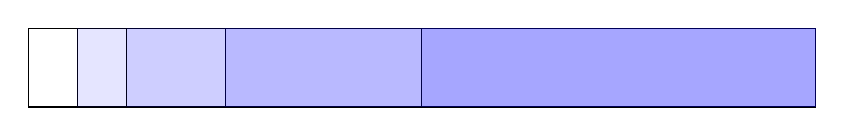
\begin{tikzpicture}[xscale=10]
		\newcommand{\buddysplit}[1]%{order}
		{
			\pgfmathsetmacro{\x}{0.5 ^ #1}
			\draw (\x, 0) -- (\x, 1);
			\fill[very nearly transparent, blue] (\x,0) rectangle (1,1);
		}
		\draw (0,0) rectangle (1,1);
		\foreach \k in {1,...,4} {
				\buddysplit{\k}
			}
	\end{tikzpicture}
	\caption{\label{fig:buddy split} 伙伴系统分割示意图}
\end{figure}

\begin{figure}
	\centering
	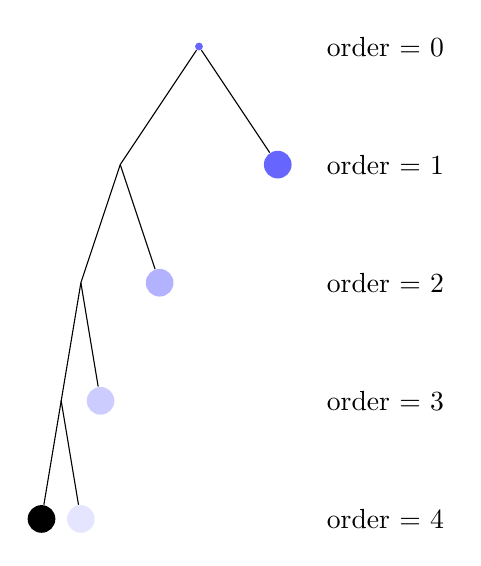
\begin{tikzpicture}
		[
			every node/.style={
					fill=blue!60,circle,inner sep=1pt,minimum width=10pt},
			level 1/.style={sibling distance=20mm,nodes={fill=blue!60}},
			level 2/.style={sibling distance=10mm,nodes={fill=blue!30}},
			level 3/.style={sibling distance=5mm,nodes={fill=blue!20}},
			level 4/.style={sibling distance=5mm,nodes={fill=blue!10}}]
		\node[minimum width=0pt] (Root) {}
		child {
				child {
						child {
								child {node[fill=black]{}}
								child {node{}}
							}
						child {node{}}
					}
				child {node{}}
			}
		child {node{}};
		\begin{scope}[every node/.style={right}]
			\xdef\level{Root}  % Initial top level
			\def\rightmostnode{Root-2}   % Name of the node with greater x coordinate
			\foreach \order in {0,...,4}
				{
					\path (\level -|\rightmostnode)
					++(5mm,0) node {order = \order};
					\xdef\level{\level-1}
				}
		\end{scope}
	\end{tikzpicture}

	\caption{\label{fig:buddy split tree} 伙伴系统分割树型示意图}
\end{figure}

若调用者需要释放之前分配的页面,分配器会找到它的伙伴(见Listing~\ref{lst: find_buddy_pfn}),如果伙伴空闲,
则把要释放的块和它的伙伴合并,并且把该伙伴从空闲列表中删除.
然后继续寻找新合成的块的伙伴,尝试合并,直到伙伴不空闲或没有伙伴,无法合并为止.
最后把合并而来的内存块加入到对应次的空闲列表中.
合并是分割的逆过程,图~\ref{fig:buddy split}和图~\ref{fig:buddy split tree}
在合并伙伴的过程中仍然适用.

伙伴系统可以达到很高的内存利用率,在模拟中可以在无法分配之前达到95\%的利用率.
而且,伙伴系统不仅无需定期的压缩和移动来减少碎片,
出现分割和合并操作的频率也很低,
总体上使用得最频繁的大小的块也是最多的.\cite{taocp1}

\begin{readsrcbox}{Buddy system}
	伙伴系统分配器的实现主要在 \linuxsrc{mm/page_alloc.c} 中.

	各种分配内存的函数最终都会调用 \lstinline{__get_free_pages()} 函数,
	通过向其传递不同的选项(GFP flags)来控制分配器的行为.
	最终进行分配的函数是 \lstinline{rmqueue()}.
	它寻找最小的空闲块,并调用 \lstinline{expand()} 来对较大的空闲块进行分割.

	处理释放工作的是函数 \lstinline{__free_one_page()},
	它负责释放块,合并伙伴,更改空闲队列.
\end{readsrcbox}

\subsection{slab 分配器}
使用伙伴系统的页面分配器是Linux内核的最底层的内存分配系统,
在页面分配器的层次之上,还有更精细的内存分配机制.
Linux内核采用slab分配器来为内核中常用的多种需要动态分配的对象管理内存.
\index{slab allocator}
在slab分配器中,同种对象连续地存储在一起,批量地分配内存,
有状态的对象在释放和分配之间,状态仍缓存在原来的空间中.
批量存储同样的对象有助于提高空间利用率、减小了内碎片化程度,
而状态的缓存则避免了频繁初始化的开销.
\cite{bonwick1994slab}
\begin{qbox}{什么是对象?}
	slab分配器管理的对象可以是存储状态的某种控制块,如进程控制块、inode等.
	也可以是无状态的缓冲区等.\index{kernel object}
\end{qbox}

在slab分配器中,对象存储在cache中,
每种对象都有自己的cache\index{slab allocator!cache},
每一个cache中又有若干slab.\index{slab allocator!slab}
slab是一小段连续的空间,通常为就为一个页面,
要分配的对象就连续地存放在slab中.
slab的分配过程中,内部的所有对象就都完成了初始化,
所以从slab中分配得到的对象永远都是已经初始化的,
调用者在分配和释放的时候既不用重新初始化也不用做全部的清理工作,
清理工作会在整个slab被销毁的时候进行.
这样的设计是考虑到有些对象的初始化开销甚至大于分配内存的开销,
保留共用的初始状态可以显著减少由于反复初始化而带来的性能损失.\cite{bonwick1994slab}

借助slab还可以减少内碎片化程度.
slab根据存储对象的状态被分为三种:
\begin{itemize}
	\item 存满对象的;
	\item 存有对象但没有装满的;
	\item 没有存储对象的,全部空闲的;
\end{itemize}
在分配新的对象时,若有没装满的slab,一定使用没装满的slab,而不引入新的碎片;
只有在没有部分装满的slab时,才会使用空闲的slab或者分配新的slab.

\begin{readsrcbox}{Slab allocator}
	slab分配器的实现在 \linuxsrc{mm/slab.c}.
\end{readsrcbox}

%%% Local Variables:
%%% mode: latex
%%% TeX-master: "linux_zh"
%%% End:


\section{设备管理}
\subsection{设备驱动模型}
计算机的CPU通过总线连接到设备,设备驱动程序通过总线与设备沟通,
并给其他部分暴露出友好的接口.
为总线、设备、驱动的相互操作而建立的程序框架在Linux内核中被称作设备驱动模型.
\cite{devicemodel}\cite{bovet2005understanding}

设备模型是由一系列相互联系的对象表示的.
表示总线、设备、驱动等的对象之间相互连接,构成层次关系,以便相互操作.
把它们连接起来的是 \lstinline{struct kobject},\index{k@\lstinline{kobject}}
一个嵌入其他结构体中提供功能的结构
(嵌入的机制与 \ref{process identifiers} 中的 \lstinline{list_head} 一样),
这其实是为了在C语言的简单结构下实现几个较复杂功能的一系列hack.

\lstinline{kobject} 接口提供的主要功能有\cite{kobject}:
\begin{itemize}
	\item 引用计数. 因为设备驱动模型对象之间相互引用的关系较复杂,
	      需要引用计数来确定对象的生命周期.
	\item 在需要释放对象时,根据对象的类型调用自定义的释放函数.
	\item 连接其他 \lstinline{kobject}.
	      设备和设备等之间需要构成父子关系.
	      不同对象之间还可以利用 \lstinline{kset} 或 \lstinline{klist} 构成collection.
	      collection 和父子关系构成了 \lstinline{kobject} 的层次结构.
	\item 向用户空间提供接口.
	      \lstinline{kobject} 在内核登记后就对应sysfs 虚拟文件系统
	      (Arch Linux下挂载在 \lstinline{/sys})下的一个目录.
	      用户态程序可以通过该虚拟文件系统的接口访问内核内部的对象.
	\item 事件的发送. 对象状态更改(如设备插拔)时可以向用户空间发送事件.
\end{itemize}
利用这些功能,内核就能构建一个灵活的设备驱动模型.

\subsubsection{总线}
总线由 \lstinline{struct bus_type} 表示.
\index{d@\lstinline{struct bus_type}}
所有设备在逻辑上都连在某一个总线上,所有驱动都要依靠总线访问设备.
因此总线的对象中的 \lstinline{struct subsys_private *p}
有两个装着 \lstinline{kobject} 的 \lstinline{kset},
分别引用该总线上的\emph{设备}和\emph{驱动}.

总线对象定义了总线普遍支持的操作,初始化具体的总线对象时要注册这些操作的函数指针,
其中一些操作是做一些总线相关的工作再调用设备的回调函数.
主要的操作有:
\begin{itemize}
	\item 在加入新的设备或驱动的时候调用的操作.
	      \begin{itemize}
		      \item 检查总线上的某个指定设备是否与指定驱动相匹配;
		      \item probe,调用驱动的probe来把设备加入到驱动的管理中;
		      \item ……
	      \end{itemize}
	\item 设备从总线上移除后的操作.
	\item 为设备准备DMA的操作.
	\item 管理设备电源、功耗的操作.
\end{itemize}

总线下的层次结构可以在sysfs 中看到.
每一种总线都在 \lstinline{/sys/bus/} 下有自己的目录.
目录下的 \lstinline{devices} 子目录是总线设备,
为指向全局的 \lstinline{devices} 子系统中的设备对象的符号链接;
\lstinline{drivers} 子目录下是总线的各个驱动.
例如 Listing~\ref{lst: pcie sysfs} 所示.

\begin{lstlisting}[caption={PCIE总线在sysfs中的结构}, label={lst: pcie sysfs}]
/sys/bus/pci-express
|-- devices
|   |-- 0000:00:07.0:pcie001 -> ../../../../devices/pci...
...
|   `-- 0000:00:1c.0:pcie010 -> ...
|-- drivers
|   |-- aer
|   |-- dpc
|   |-- pciehp
|   `-- pcie_pme
|-- drivers_autoprobe
|-- drivers_probe
`-- uevent
\end{lstlisting}

\subsubsection{设备}
设备在Linux设备驱动模型中的对象为 \lstinline{struct device}.
\index{d@\lstinline{struct device}}
其中存储的一些信息有:
\begin{itemize}
	\item 设备的名字;
	\item 设备的“父设备”,例如总线控制器、hub控制器等;
	\item 设备所在的总线类型;
	\item 设备使用的驱动;
\end{itemize}

\begin{qbox}{总线也是设备吗?}
	值得注意的是虽然已经有表示总线类型的 \lstinline{bus_type},
	总线也还是作为设备在设备驱动模型中表示,
	一种总线可能是另一种总线的子设备,
	例如挂在 PCI-E 总线下的 USB 总线.
\end{qbox}

\subsubsection{驱动}
设备驱动的对象是 \lstinline{struct device_driver}.
\index{d@\lstinline{struct device_driver}}
一个驱动对象只能存在一个实例,
也就是说驱动只有一份,一个驱动要管理与其关联的所有设备.
所以 \lstinline{struct device_driver} 的 \lstinline{struct driver_private *p}
要存储当前驱动所管理的所有设备.

向驱动添加设备的机制是存储在 \lstinline{struct device_driver} 中的函数指针
\lstinline{probe()}.\index{p@\lstinline{probe()}}
这个函数以 \lstinline{struct device} 为参数,应该做这样几件事\cite{devicedriver}:
\begin{itemize}
	\item 确定设备确实存在;
	\item 确定设备的型号和版本能被驱动支持;
	\item 为设备需要的数据结构分配内存空间;
	\item 初始化设备的硬件;
	\item 最后把设备驱动和设备绑定在一起,填上各自的引用.
\end{itemize}
\index{d@\lstinline{struct device}}
\begin{readsrcbox}{设备驱动模型}
	总线的表示 \lstinline{struct bus_type}\index{d@\lstinline{struct bus_type}}
	的定义在 \linuxsrc{include/linux/device/bus.h}.
	实际的总线定义自己的 \lstinline{struct bus_type},
	如PCI的 \lstinline{struct pci_bus_type} 在 \linuxsrc{drivers/pci/pci-driver.c}.

	设备的 \lstinline{struct device}\index{d@\lstinline{struct device}}
	定义在 \linuxsrc{include/linux/driver.h}.
	往往 \lstinline{struct device} 不单独使用,
	特定总线的设备会把 \lstinline{struct device} 嵌入在一个有更多信息的结构体中.
	比如PCI的 \lstinline{struct pci_dev} (\linuxsrc{include/linux/pci.h})、
	USB的 \lstinline{struct usb_dev} (\linuxsrc{include/linux/usb.h}).

	驱动的 \lstinline{struct device_driver} \index{d@\lstinline{struct device_driver}}
	在 \linuxsrc{include/linux/device/driver.h}.
	同样特定总线的驱动会把 \lstinline{struct device_driver} 嵌入到自己定义的结构体中.
\end{readsrcbox}

\subsection{设备驱动过程}
在 \ref{loading modules} 中,我们提到内核启动时,
bootloader加载vmlinux镜像,内核代码开始运行.
在开始启动init进程和运行init程序之间,
内核首先做最核心的初始化,这其中就包括设备驱动模型的初始化.
系统的总线等重要的设备的内核模块是静态连接到 vmlinux 内的,
在设备驱动模型初始化完成后,
这些模块的初始化程序会运行,注册对应的设备和总线类型,对总线进行初始化并设置中断.
这样基本的驱动框架就建立好了,总线的设备驱动就可以对总线上的设备进行搜索.
每当找到一个新的设备,首先初始化相关的对象,
然后通过总线的 \lstinline{match()} 和驱动的 \lstinline{probe()}
来遍历该总线下的所有驱动,如果发现匹配的驱动,则停止遍历,
把设备和驱动绑定起来,这样设备模型的总线、设备、驱动就都联系起来了.

现在再把用户空间的操作考虑进去.
嵌有 \lstinline{kobject} 的设备、驱动对象
在创建、删除的时候都会向用户空间传递 \lstinline{uevent}.
用户空间的程序可以通过监听事件,并且通过 sysfs 对设备驱动模型进行操作,
从而支持更灵活的设备使用方式,如热插拔.
在用户态受限的环境下管理设备的好处还有稳定性和安全性的提高.
同样在 \ref{loading modules} 中提过,
包括 Arch Linux 在内的大多数x86发行版都使用systemd的udev\index{udev}
系统来在用户态管理设备.
udev负责监听 \lstinline{uevent} 事件,
根据udev自带的和用户自定义的规则来做出对应的动作,
管理 \lstinline{/dev} 下的 device node 文件,
使其他程序可以通过 \lstinline{/dev} 下的文件与设备驱动程序交互.
udev规则一般可以实现这样的一些功能\cite{WritingUdev}:
\begin{itemize}
	\item 加载、卸载驱动所在的模块(见 \ref{loading modules}).
	\item 在 \lstinline{/dev} 下为设备设置友好的名字.
	\item 通知其他程序,传递设备的事件.
	\item 进行系统管理,如挂载刚刚插入的硬盘.
\end{itemize}

使用udev的命令行工具 \lstinline{udevadm} 可以直观地看到设备状态变化产生的操作.
比如运行 \lstinline{udevadm monitor --property} 命令,插入一个USB键盘,就可以看到udev根据规则和事件创建的device node.

\begin{lstlisting}
UDEV  [401515.997363] add      /devices/pci0 ... /usb3/.../event12 (input)
ACTION=add
DEVPATH=/devices/ ... /usb3/ ... /event12
SUBSYSTEM=input
DEVNAME=/dev/input/event12
\end{lstlisting}

\begin{notebox}
	这里描述的过程进行了大量的简化,许多重要的细节都忽略了.
	例如驱动可能在 \lstinline{probe()} 时还为准备好,
	这时它可以要求推迟 \lstinline{probe()} 的操作.
\end{notebox}

\begin{readsrcbox}{\lstinline{driver_init()}}
	初始化设备模型的函数入口为 \lstinline{driver_init()},
	位于 \linuxsrc{drivers/base/init.c},
	由 \linuxsrc{init/main.c} 中的 \lstinline{do_basic_setup()} 调用.
	\linuxsrc{drivers/base} 目录为内核驱动的“core”部分,
	负责硬件驱动模型内部的初始化和实现模型内部的功能等.

	\linuxsrc{drivers/base/core.c} 中的 \lstinline{device_add()}
	处理添加设备时的一系列操作,
	调用 \lstinline{bus_probe_device(dev);} 来匹配驱动.
	\lstinline{bus_probe_device()} 位于 \linuxsrc{drivers/base/dd.c},
	dd是“device/driver”的缩写,该文件中的函数处理设备和驱动之间的关系,
	例如绑定、通信等.
\end{readsrcbox}
%%% Local Variables:
%%% mode: latex
%%% TeX-master: "linux_zh"
%%% End:


\section{ext4文件系统}
ext4\index{ext4}是近年许多GNU/Linux发行版的默认文件系统,于2008年在内核中稳定
\footnote{\url{https://git.kernel.org/?p=linux/kernel/git/torvalds/linux-2.6.git;a=commit;h=03010a3350301baac2154fa66de925ae2981b7e3}},
是较为传统的日志文件系统,而不是BTRFS、ZFS那样的集成了卷管理器的文件系统,
但功能也较为完善.

\subsection{磁盘空间和文件的组织}
\subsubsection{存储单元}
ext4中,磁盘的空间被分为几种单位:sector、block和block group.
\begin{itemize}
	\item sector 是由硬盘决定的扇区,一般为512 B.\index{sector}
	      较新(2010后)硬盘一般扇区大小为4096 B,
	      可以工作在4 KB 的原生扇区大小模式下,
	      也可以模拟512 B的扇区大小.
	\item block 是2的整数次幂个连续扇区组成的单元,\index{block}
	      一次传输较多数据可以减小磁盘操作开销.
	      一般是4 KB,为了匹配常见的内存页面的大小.
	      默认开启64位特性时,一个文件系统可以有 $2^{64}$ 个block.
	\item block group 是连续的block,默认为32768个block. \index{block group}
	      ext4会利用block group来提高局部性.
\end{itemize}
值得注意的是,在引用内存中的数据时,指针为按字节寻址的地址,
也就是引用对象的第一个字节的字节数;
而在外存中,存储单元为block,所以指针均为block number.
还有一点,因为文件系统不应依赖CPU的类型,
所以应该定义好所有的数据的字节序.
ext4中除日志外的数据均为little-endian.

\subsection{文件的组织形式}
文件的数据部分存储在数据block中,而要想把数据block组织成一个文件,
还需要一些辅助用的block.
ext4的空间分配方式为索引式,也就是组成文件的块可以不连续,
用inode来索引分配给文件的块.
inode 其实就表示了文件的连续的逻辑块号到不连续的物理块号的一个映射,
和页表在虚拟内存中的作用类似.

inode中存有文件的元数据和一些能够索引到数据block的数据结构.
普通的索引方式是直接或间接地存储每一个block的指针.
直接索引的block有12个(\lstinline{EXT4_NDIR_BLOCK}),
这12个指针的后面是3个指向间接索引块的指针,
分别为一级、二级和三级间接索引.
15个指针共有60个字节,存放在 \lstinline{i_block} 字段中.
小的文件不需要间接索引块,而如果文件的数据块超过12个,
就需要分配间接索引块,若一级间接索引仍不够再依次使用二级索引、三级索引.
若block大小为4 KB,则每一个间接块可以存放32位指针
(这里只能用32位的block nunber)的数量为 $4\times2^{10}/4 = 2^{10}$.
故全部的二级索引块可以索引 $2^{10}\times2^{10}\times\SI{4}{\kilo\byte} = \SI{4}{\giga\byte}$.
可以看出,只有数GB的文件才要用到三级间接索引.

另外一种方式是extent.
这是一种介于连续分配和索引之间的组织方式,可以弥补两者的不足.
分配时,尽量分配连续的block,但是确实无法分配连续的空间时,
也可以用分开的若干个连续区域来存储,每一个连续的空间称为一个extent. \index{extent}
为了在连续的逻辑块号和这样的部分连续的物理块号之间建立索引,
Linux采用的是extent tree,一种类似于B+ 树的索引结构.
我们在数据结构课上学过,B+ 树是一种多分支的自平衡树,
树中的元素都是叶子节点,非叶子节点只用于索引,
extent tree 也是这样.
每一个extent 记录起始块号和长度,树的叶子节点就是extent.
索引方式下存储指针的位置,
extent方式则存放extent树.
extent树的每一个节点都有一个header描述这个节点可索引多少个extent,
已经有多少extent等信息.
如果inode的那60个字节可以放下一个header和所有extent,
则不需更多块来存放节点.
如果放不下,则要使用索引节点来间接指向extent.\cite{Ext4Extent}

\lstinline{i_block} 的60个字节除了存放块索引和extent tree,\index{extent tree}
还可以存放符号链接的目标路径,若存不下,还需分配更多空间.

目录也是文件的一种,同样由inode索引.
与其他文件不同的是,目录文件的数据块存放的是目录中每一个文件或目录的条目,
ext4中,每一个文件的目录条目包含:
\begin{itemize}
	\item 文件名字符数组、文件名长度(不超过255);
	\item 文件的inode号;
	\item 文件类型;
\end{itemize}
其中文件类型也在inode中存在,在目录条目复制一份的好处是,
查看目录下所有文件类型时无需访问每一个文件的inode,
只需要查看所有条目即可.\cite{ext4dynamic}
目录条目除了顺序存储,还可以组织成更复杂但高效的htree(hashed btree). \index{htree}
在这种组织形式下,用名字访问文件的时间复杂度更低,
只需用文件名的散列值作为索引在B树中搜索.


%%% Local Variables:
%%% mode: latex
%%% TeX-master: "linux_zh"
%%% End:


\section{附录}
\tcblistof[\subsection]{question}{“小问题”列表}
\tcblistof[\subsection]{src}{“读源码”列表}

\printbibliography[heading=bibintoc]

\printindex

\newpage

\end{document}

%%% Local Variables:
%%% mode: latex
%%% TeX-master: t
%%% End:
